\chapter{A semi-empirical model point of view} \label{ch:SEM}

%\begin{center}
%  {\it ``If could add an introductionary text here.''}
%  \vspace{1cm}
%\end{center}

In this Chapter we exploit semi-empirical models (SEMs), which are a competitive, fast and flexible methodology, extensively used in recent years to constrain the degree of evolution and mergers in galaxies, as well as the degree of coevolution with their central BHs \citep{2013ApJ...762...70C, 2019MNRAS.487..275G, 2019MNRAS.487.2005C, 2020arXiv201002957A}. The aim of SEMs is to generate large mocks of normal and 
active galactic nuclei (AGN) host galaxies
%active galaxies 
on top of large dark matter halo catalogs, relying on only a few observationally-motivated inputs. Part of this work has been submitted as a letter to the Monthly Notices of the Royal Astronomical Society.

We use SEMs to explore a variety of input relations in our model and show that the L$_{\rm X}-{\rm M}_{*}$ relation naturally arises from the underlying dependence of BH mass (M$_{\rm BH}$) and SFR on M$_*$. More specifically, its slope and normalization are fully determined by, respectively, the M$_{\rm BH}-{\rm M}_*$ scaling relation and the characteristic Eddington ratio distribution.

In Section~\ref{sec:model} we present our model and in Section~\ref{sec:results} we highlight the main parameters controlling the L$_{\rm X}-{\rm M}_*$ evolution at different redshifts and  galaxy phases.
In Section~\ref{sec:disc_concl} we discuss our findings and draw our conclusions on their relevance to the galaxy-BH co-evolution. %Throughout this paper we assume a \citet{2003PASP..115..763C} initial mass function and a flat cosmology with $H_0=70$~Km/s/Mpc, $\Omega_\lambda=0.7$, $\Omega_0=0.3$.

\section{Building robust AGN mock catalogs}\label{sec:model}
In this study, we create realistic mock catalogs of AGN and non-active galaxies to study which input parameters mostly control the L$_{\rm X}$ - SFR relation at different redshifts. We here below provide the most relevant steps in the generation of our mocks, and refer the reader to \citet{Allevato21} for full details.

We start from a halo distribution generated via a halo mass function from \citet{2008ApJ...688..709T} at the redshift of interest. To each dark matter halo we assign a galaxy stellar mass according to the stellar - halo mass relation of \citet[][]{moster10} with updated parameters from \citet[][Eq.~5]{2019MNRAS.483.2506G} with a normal scatter in stellar mass at fixed halo mass of $0.11$~dex.
We then assign a BH mass via the M$_{\rm BH}-{\rm M}_*$ calibrated by \citet{2015ApJ...813...82R}, with an intrinsic scatter of $0.55$ dex, and also explore the impact of adopting other M$_{\rm BH}-{\rm M}_*$ relations from \citet{2016MNRAS.460.3119S}, \citet{2018ApJ...869..113D} and \citet{2019ApJ...876..155S}, which bracket the systematic uncertainties in the BH-galaxy stellar mass in the local Universe. 
We then assume that each relation does not evolve with redshift, as suggested by a number of recent studies \citep[e.g.][and Fig.~\ref{fig:comp_models}]{2019ApJ...885L..36D, Suh20, Shankar20MNRAS}.
To each galaxy and BH we then assign an Eddington ratio $\lambda\equiv L_{bol}/L_{\rm Edd}$ and convert bolometric luminosities $L_{bol}$ to 2-10 keV X-ray luminosities $L_X$ via the same bolometric corrections $k_X$ adopted in Chapter~\ref{ch:observations} (see Sec.~\ref{subsec:LX_BHAR}). Following the formalism in, e.g., \citet{Shankar13Acc} and \citet{Allevato21} and references therein, which follows the one routinely adopted in continuity equation models, the AGN luminosity function is given by the convolution
\begin{equation}
\Phi(\log L_{bol},z)=\int_{\log \lambda_{\rm min}}^{\log \lambda_{\rm max}}U(y,z) n(y,z) P(\log \lambda,z)d\log \lambda \, 
\label{eq:PhiL}
\end{equation}
%\begin{equation}
%\Phi(\log L,z)=\int_{\log \lambda_{\rm min}}^{\log \lambda_{\rm %max}}U(\log {\rm M}_{\rm BH},z)\times n(\log {\rm M}_{\rm %BH},z)\times P(\log \lambda,z)d\log \lambda    
%\end{equation}
where $y=\log {\rm M}_{\rm BH}$, $P(\log \lambda,z)$ is the average Eddington ratio distribution of active sources normalized to unity, which we assume for simplicity to be independent of BH mass, and $n(y,z)$ is the total BH mass function. $U(y,z)$ is the duty cycle, i.e. the fraction of active sources of a given mass at a given epoch accreting in the range $\log \lambda_{\rm min}<\log \lambda<\log \lambda_{\rm max}$. We fix our minimum Eddington ratio to $\log \lambda_{\rm min}=-4$ to include the lowest X-ray luminosities recorded in the AGN luminosity function, i.e. $L\sim 10^{40}\,$ erg/s for M$_{\rm BH}\gtrsim 10^6 \, M_{\odot}$, and set $\log \lambda_{\rm max}=1$, though the exact values of $\log \lambda_{\rm min}$ and $\log \lambda_{\rm max}$ do not alter any of our results. The flexibility offered by Eq.~\ref{eq:PhiL} allows to disentangle the effects of the shape of $P(\log \lambda,z)$, which carries information on the accretion properties of a BH, from the fraction $U(y,z)$ of active BHs above a certain threshold in luminosity/Eddington ratio. The reference $P(\log \lambda,z)$ distribution is taken to be a simple Gaussian in $\log \lambda$ characterized by a standard deviation $\sigma$ and a mean $\mu$. We will show that the shape of the $P(\log \lambda,z)$ distribution plays a minor role in the outputs as long as the characteristic Eddington ratio, defined as
\begin{equation}
\zeta_c(z)\equiv<\log \lambda>(z)=\int_{\log\lambda_{\rm min}}^{\log \lambda_{\rm max}} P(\log\lambda,z)\log(\lambda) \,d\log(\lambda)\, ,
\end{equation}
is the same.
We take the duty cycle empirically inferred by \citet{2010A&A...516A..87S} and \citet{2015MNRAS.447.2085S}, decreasing with M$_{\rm BH}$, and also experiment with the ones proposed by \citet{2019MNRAS.488...89M} and \citet{2017MNRAS.471.1976G}, increasing with M$_{\rm BH}$, and a constant duty cycle as suggested by \citet{goulding10}. 
We assign SFRs to quiescent, normal star-forming, and starburst galaxies based on their respective SFR-M$_*$ relation.
For starburst and quiescent galaxies, we adopt the SFR fits from Table~\ref{table:all_fitpar}, while for the ``main sequence'' we adopt the 
\citet[Eq.~9]{2015A&A...575A..74S} flexible parametric formula
\begin{equation}
    \log_{10}\left(\frac{\rm SFR}{M_\odot yr^{-1}}\right)= m - m_0 +a_0 r - a_1[\max(0,m-m_1-a_2r)]^2
	\label{eq:SFR}
\end{equation}
with $m\equiv\log_{10}(M_*)-9$ and $r\equiv\log_{10}(z+1)$. Best-fit parameters for the data are $a_0=2.29\pm 0.12$, $a_1=0.25 \pm 0.04$, $a_2=0.33 \pm 0.30$, $m_0=0.64 \pm 0.03$, $m_1=0.55\pm 0.11$, and the fit is shown in Fig.~\ref{fig:SFR_2D_fit}. We add a dispersion of $0.2$~dex to the SFR. 
\begin{figure*}
%%%%%\vspace{8cm}
\begin{center}
  %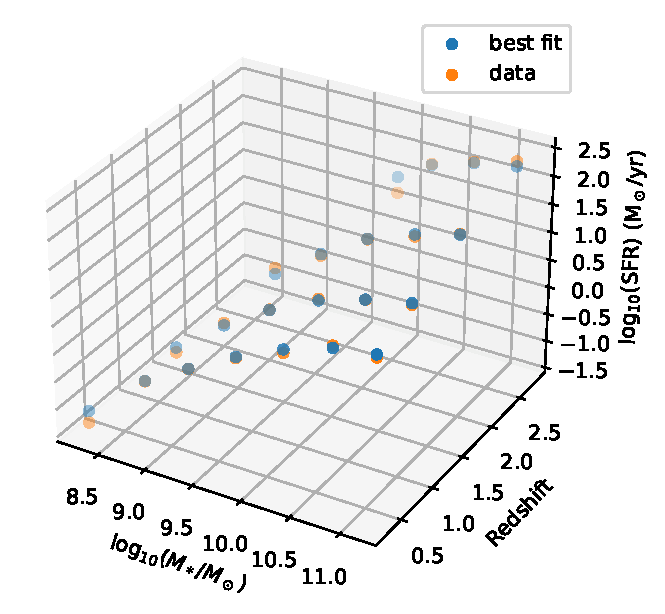
\includegraphics[trim={2cm 13.5cm 0.3cm 0.5cm},
  \includegraphics[width=0.65\linewidth]{Figs/Chapter3/2D_SFR_fit_data.pdf}
  \caption{A 2-dimensional plot of the SFR data for star forming galaxies from Chapter~\ref{ch:observations} as a function of ${\rm M}_*$ and redshift, compared with our best fit of Eq.~\ref{eq:SFR}.
  }
    \label{fig:SFR_2D_fit}
\end{center}
\end{figure*}
\begin{figure*}
%%%%%\vspace{8cm}
\begin{center}
  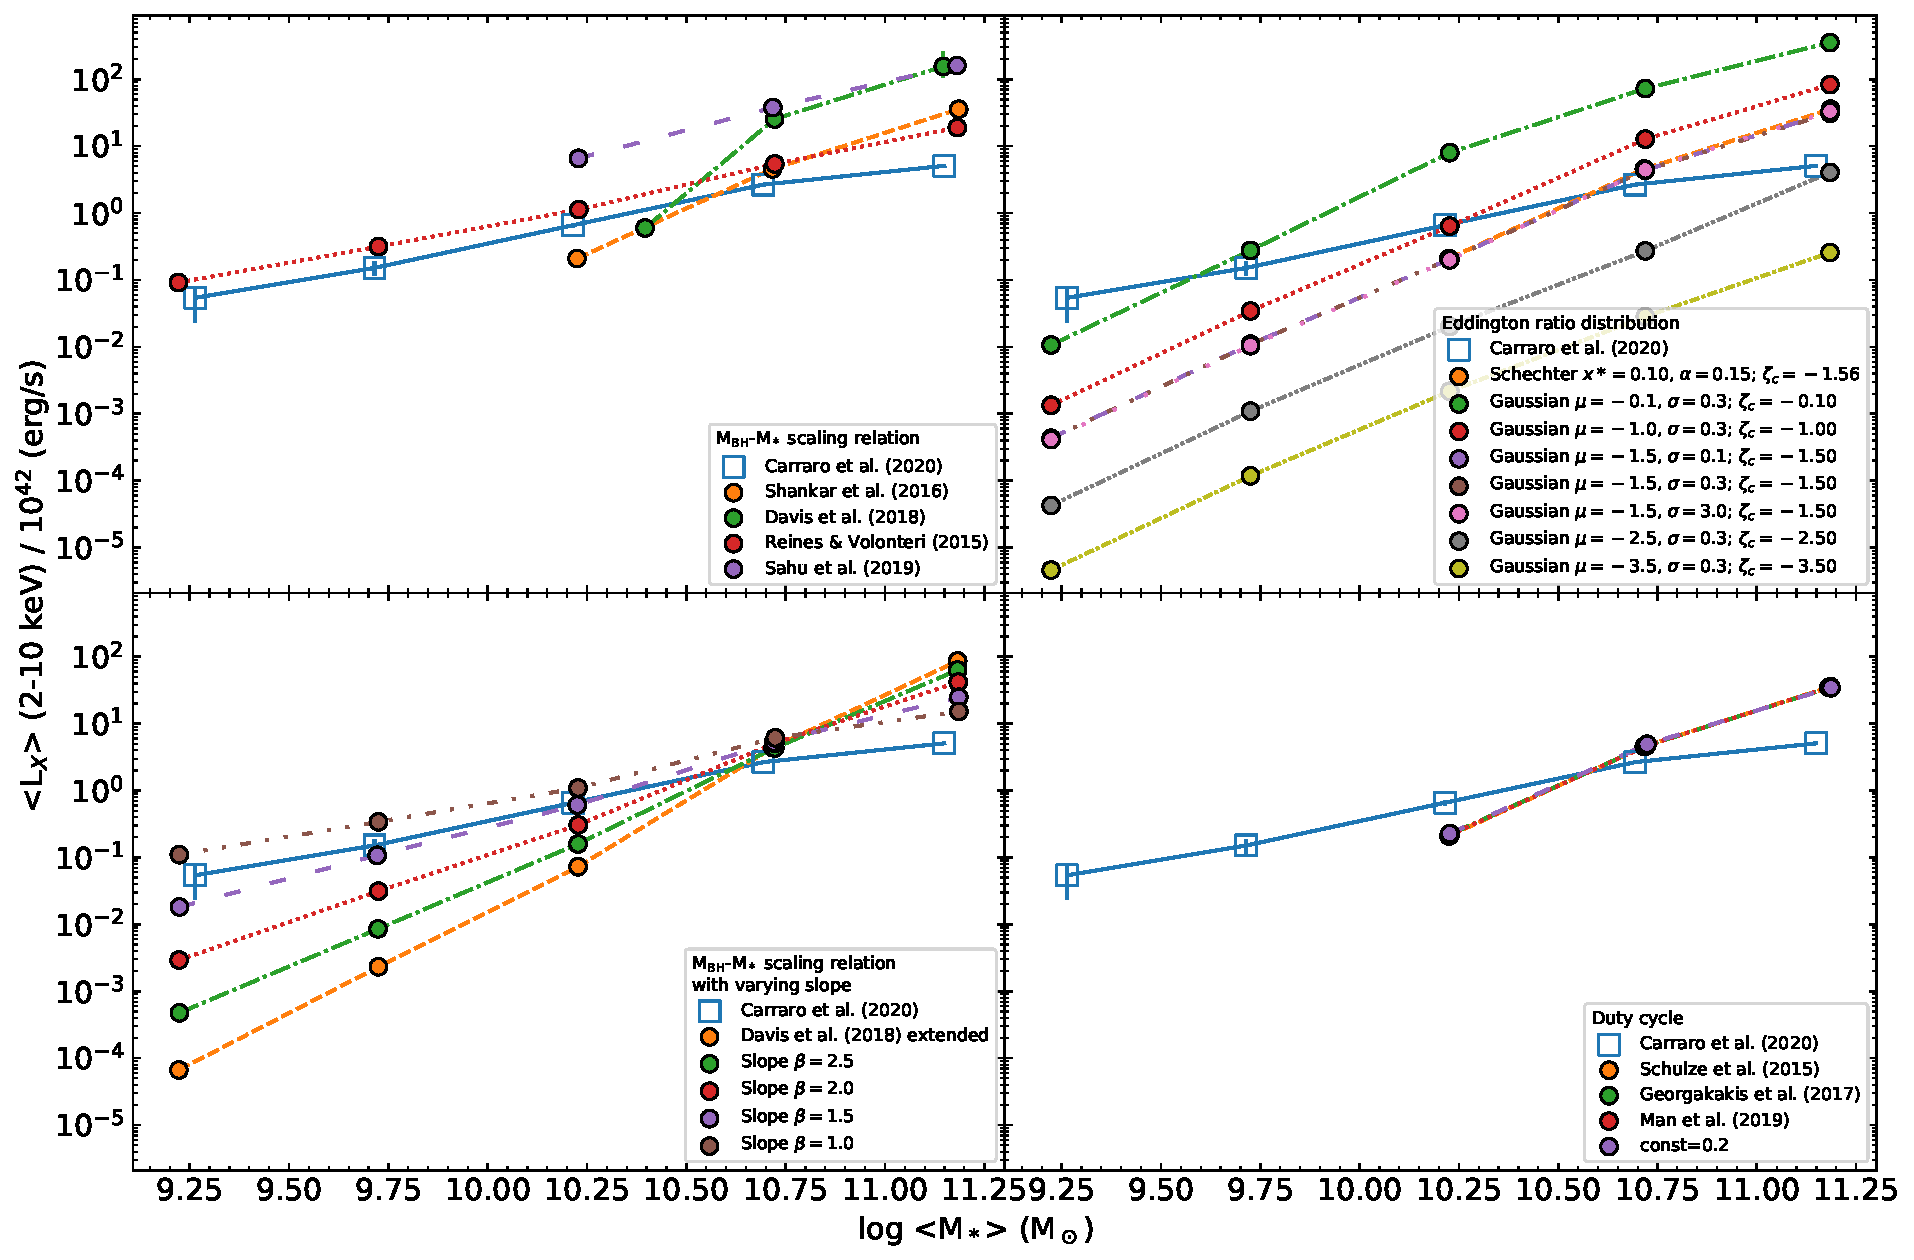
\includegraphics[width=\textwidth]{Figs/Chapter3/fig2_z1.0.pdf}
  \caption{A gallery of L$_{\rm X}-{\rm M}_*$ relations obtained by varying one of the input relations at a time. The relation that varies in each subplot is reported in the legend. 
  %Broken lines are added to the plot to guide the reader. All data-points are at $z=1$.
  Results from COSMOS data at $z=1$ from Chapter~\ref{ch:observations} (blue squares, see Fig.~\ref{fig:L_X}), are included in all plots for comparison.
  %All data-points are at $z=1$.
  Top left: L$_{\rm X}-{\rm M}_*$ relation obtained by changing the Eddington ratio distribution function. We use a Schechter function and Gaussian function in $\log(\lambda)$ with varying mean $\mu$ and standard deviation $\sigma$ values.
  Top right: L$_{\rm X}-{\rm M}_*$ relation obtained by changing the duty cycle method. Each M$_{\rm BH}-{\rm M}_*$ scaling relation is shown within its original stellar mass range of derivation.
  Bottom left: L$_{\rm X}-{\rm M}_*$ relation obtained by changing the M$_{\rm BH}-{\rm M}_*$ scaling relation.
  Bottom right: L$_{\rm X}-{\rm M}_*$ relation obtained with a toy M$_{\rm BH}-{\rm M}_*$ scaling relation where we change the logarithmic slope $\beta$ of the relation $\log {\rm M}_{\rm BH} = \alpha + \beta \log {\rm M}_*$.
  }
    \label{fig:LX_M}
\end{center}
\end{figure*}
Before computing the average X-ray luminosity we assign to each galaxy, irrespective of their duty cycle, an X-ray luminosity from X-ray binary emission following \citet[][Table 3]{2016ApJ...825....7L}, and then, as in Sec.~\ref{subsec:LX_BHAR}, subtract the mean binary emission competing to that bin of stellar mass and star formation rate. We note that neglecting X-ray binary emission entirely from our procedure would yield very similar results.
Following the procedure described above, we generate diverse galaxy mock catalogs with distinct choices of the input scaling relations, duty cycles, and $P(\log\lambda,z)$ distributions. 
We then divide each AGN mock catalog in bins of stellar mass, and perform 500 bootstraps out of which we extract the median SFR and M$_*$, and the linear mean L$_{\rm X}$ weighted by the AGN duty cycle %\log M_{BH,i}
\begin{equation}
\left<L_X\right>=\frac{\sum_i U_i(y_i,z) L_X(y_i)} {\sum_i U_i(y_i,z)}\, ,
    \label{eq:meanLx}
\end{equation}
where 
\begin{equation}
\log L_X(y_i) [erg\;s^{-1}]=38.1 +\log \lambda_i +y_i-\log k_X.
\label{eq:Lx_210}
\end{equation} 
For each bootstrapped distribution we compute the median SFR and $L_X$ and their 5th and 95th percentiles, following the same procedure as in the comparison observational sample Chapter~\ref{ch:observations}.



\section{Results}\label{sec:results}

\subsection{The effect of the model's inputs on the ${\rm L}_{\rm X}-{\rm M}_*$ relation} \label{ssec:Fig2}

To pin down the input parameters that mostly control the L$_{\rm X}-{\rm M}_*$ relation, we explore in Figure~\ref{fig:LX_M} how the relation varies by changing, from top left to bottom right, the $P(\log \lambda,z)$, the duty cycle, the full M$_{\rm BH}-{\rm M}_*$ relation, and only the slope of the \citet{2015ApJ...813...82R} relation, as labeled. 
All the mocks are generated at $z=1$, though the results are applicable at all redshifts, as further discussed below.

The top panels clearly show that whilst the normalization of the L$_{\rm X}-{\rm M}_*$ relation is strongly controlled by the characteristic Eddington ratio $\zeta_c$ (left), it has a negligible dependence on the AGN duty cycle (right). To note that a Schechter or Gaussian $P(\log \lambda,z)$ yield the same mean X-ray luminosity at fixed stellar mass as long as their $\zeta_c$ are the same (dotted green and dot-dashed red lines). The mean X-ray luminosity will be mostly controlled by the rate at which galaxies of a given BH/stellar mass are accreting and not by how many galaxies are active at any given time. The bottom panels of Figure~\ref{fig:LX_M} show instead a direct proportionality between the normalizations (left) and slopes (right) of the  M$_{\rm BH}-{\rm M}_*$ and the L$_{\rm X}-{\rm M}_*$ relations: a lower/shallower M$_{\rm BH}-{\rm M}_*$ scaling relation will result in a proportionally lower/shallower L$_{\rm X}-{\rm M}_*$ relation, and vice versa.

It is clear from Fig.~\ref{fig:LX_M} that the slope and normalization of the input M$_{\rm BH}-{\rm M}_*$ relation, as well as the input $\zeta_c$, all play a significant, and in fact degenerate, role in shaping the L$_{\rm X}-{\rm M}_*$ relation. For example, a flatter slope in the M$_{\rm BH}-{\rm M}_*$ relation or a mass-dependent $\zeta_c$, progressively decreasing at larger masses, could both produce a flatter slope in the L$_{\rm X}-{\rm M}_*$ relation. A decreasing $\zeta_c$ with increasing M$_{\rm BH}$ or ${\rm M}_*$  could indeed reconcile the observational results from Chapter~\ref{ch:observations} with a steeper M$_{\rm BH}-{\rm M}_*$ relation as calibrated in the local Universe \citep[e.g.,][]{2016MNRAS.460.3119S,2018ApJ...869..113D}. 

The results reported in Fig.~\ref{fig:LX_M} point to the L$_{\rm X}-{\rm M}_*$ relation as a powerful tool to constrain the mean rate of accretion of BHs $\zeta_c$ as a function of time and BH mass in ways independent of the duty cycle. 
As detailed in Eq.~\ref{eq:PhiL}, the AGN X-ray luminosity function is degenerate in BH mass function, duty cycle and $P(\lambda,z)$. However, independent constraints on $\zeta_c$ from the L$_{\rm X}-{\rm M}_*$ relation could then shed light on the duty cycle if a robust estimate of the underlying BH-galaxy scaling relation is available from, e.g., AGN clustering measurements \citep[see discussion in][]{ShankarNat,Allevato21}, or vice versa.

\subsection{The minor effect of $\lambda_{min}$ on our models}
We are considering in our mock catalogs galaxies with an Eddington ratio in the range $-4<\log(\lambda)<1$. This limit cannot be imposed in the selection of the observational sample for obvious reasons, but the effect of this choice of the minimum Eddington ratio $\lambda_{min}$ is negligible. In fact, we can extend the distribution of Eddington ratios down to ever lower $\lambda_{min}$ and still find very similar average X-ray luminosities, as long as the starting overall shape of the Eddington ratio distribution is not changed. This behavior simply stems from the fact that, to match the observational data, we are selecting in the mock catalogs galaxy stellar masses above ${\rm M}_*\ge 10^9 {\rm M}_\odot$, which tend to correspond to BH masses of the order of ${\rm M}_{\rm BH}\ge10^5 {\rm M}_\odot$, which in turn are mapped to (minimum) X-ray luminosities of the order of ${\rm L}\ge10^{38}erg/s$ (see Eq.~\ref{eq:Lx_210}).

Extending to even lower Eddington ratios produces proportionally lower X-ray luminosities that do not significantly contribute to the mean X-ray luminosity in any stellar mass bin considered in this work. In Fig.~\ref{fig:test_lambda_min} we show the predicted  relation when varying the $\lambda_{min}$ by 4 orders of magnitude, as labeled, but keeping fixed the overall shape of the input Eddington ratio distribution, BH-galaxy scaling relation and duty cycle. 
As expected, the average X-ray luminosity is nearly identical in all cases, as the minimum X-ray luminosities tend to be the same when keeping the same cuts in stellar mass.

\begin{figure*}
\begin{center}
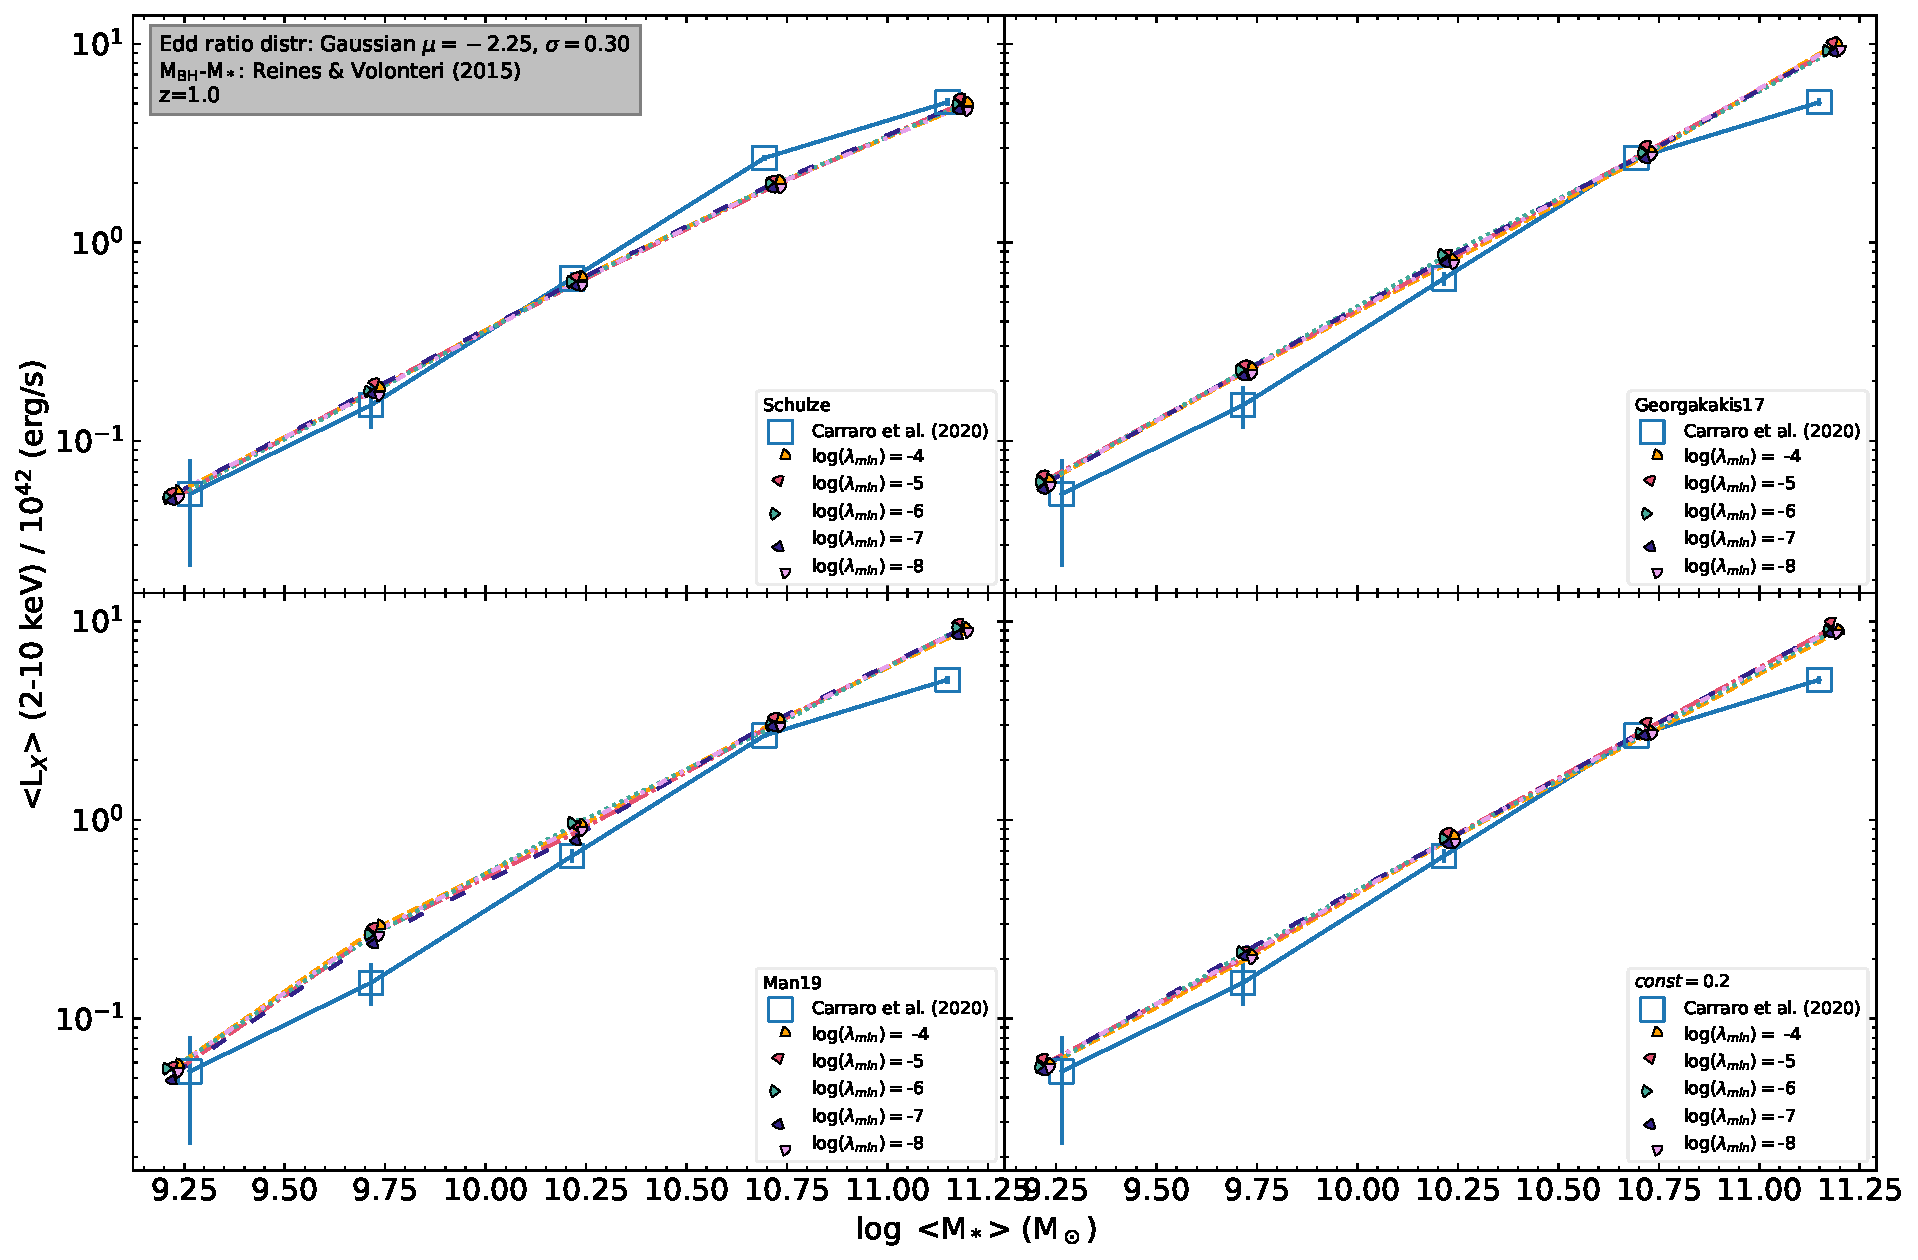
\includegraphics[width=\textwidth]{Figs/Chapter3/Test_lambda_min_z1.0.pdf} 
  \caption{L$_{\rm X}$ as a function of ${\rm M}_*$ for each of the duty cycles considered in this Chapter by varying the value of the minimum Eddington ratio, as labeled.}
    \label{fig:test_lambda_min}
\end{center}
\end{figure*}

\subsection{Reproducing the ${\rm L}_{\rm X}-{\rm M}_*$ relation through cosmic time}

In this Section we extend the comparison to data on the L$_{\rm X}-{\rm M}_*$ relation at different redshifts. The data point to a steady decrease of the mean ${\rm L}_{\rm X}$ luminosity with cosmic time at fixed host galaxy stellar mass. As discussed above, this decreasing trend could be interpreted either as a progressive decline in the normalization of the M$_{\rm BH}-{\rm M}_*$ relation and/or in the characteristic $\zeta_c$. The latest data suggest a rather weak evolution in the M$_{\rm BH}-{\rm M}_*$ relation up to at least $z\sim 2.5$ \citep[e.g.,][]{Suh20,Shankar20MNRAS} thus favoring, in our approach, a steady decrease in $\zeta_c$, which would also be in line with independent observations \citep[]{Kollmeier06} and continuity equation models \citep[][]{Shankar13Acc,Aversa15}.

In Figure~\ref{fig:LX_M_redshift} we show the L$_{\rm X}-{\rm M}_*$ relation for mock catalogs at $z=0.45,1.0,2.7$ (left, central and right panels respectively), generated by assuming as a reference the \citet{2015ApJ...813...82R} M$_{\rm BH}-{\rm M}_*$ relation, which naturally generates a slope in the L$_{\rm X}-{\rm M}_*$ relation, consistent with our data. 
 At each redshift we plot the models for two values of $\mu$ in $P(\log \lambda,z)$ (the corresponding $\zeta_c$ values are very similar being Gaussian distributions), roughly consistent with the higher and lower values of the L$_{\rm X}-{\rm M}_*$ relation.
We find that, assuming a strictly constant M$_{\rm BH}-{\rm M}_*$ relation, to reproduce the data we would need a drop of a factor of $\gtrsim 10$ in the characteristic Eddington ratio $\zeta_c$ from $z\sim 2.7$ to $z\sim 0.45$, which is broadly in line with some observational data and models' results \citep[see, e.g., Fig. 12 in][]{Shankar13Acc}. 

\begin{figure*}
%%%%%\vspace{8cm}
\begin{center}
  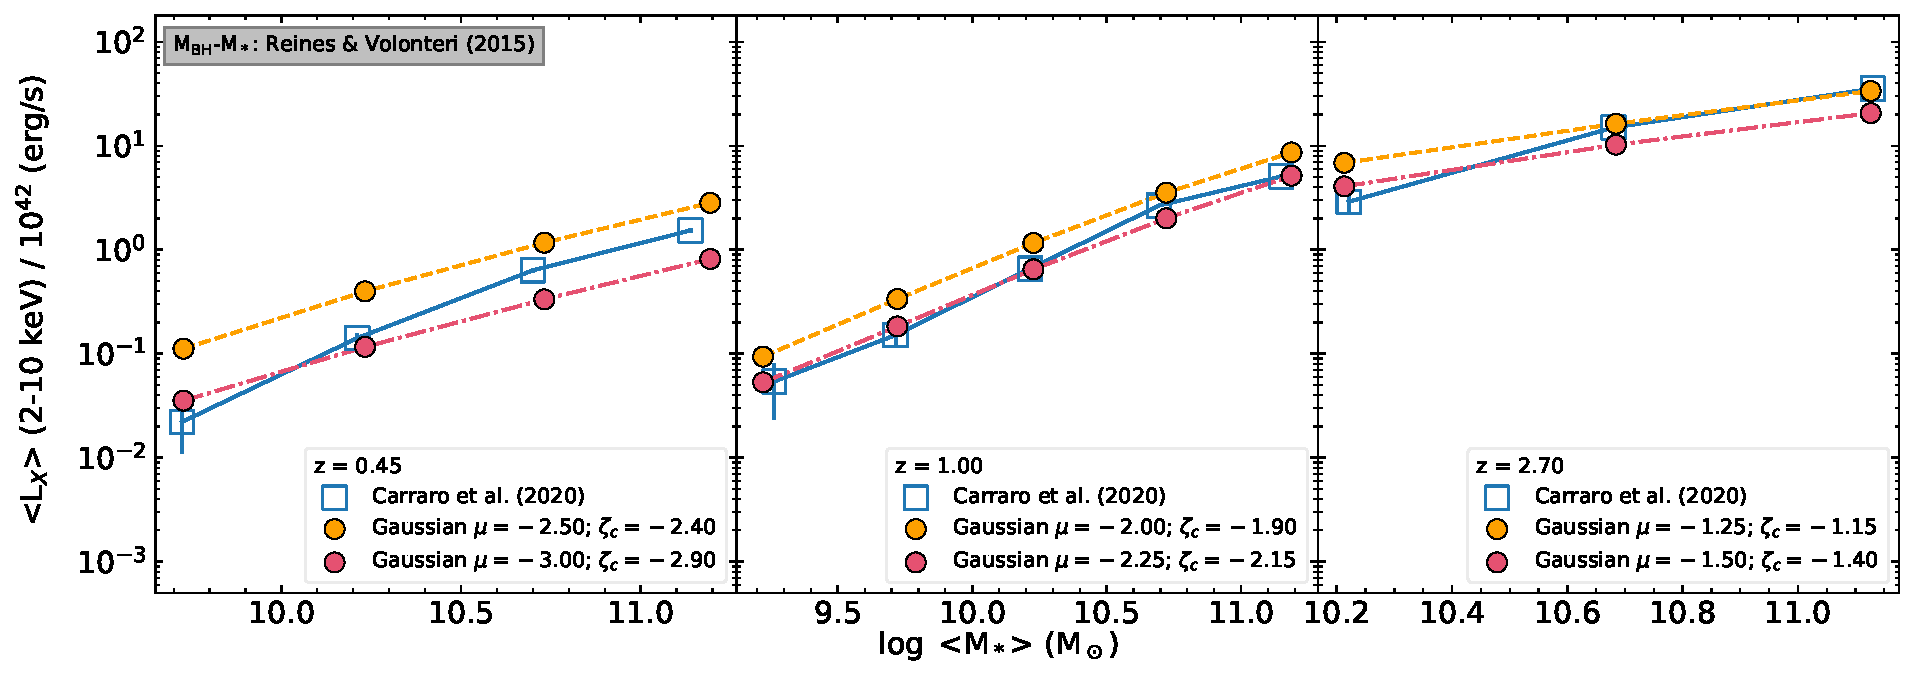
\includegraphics[width=\textwidth]{Figs/Chapter3/fig3.pdf}
  \caption{The L$_{\rm X}-{\rm M}_*$ relations at $z=0.45$ (left panels), $z=1.0$ (central panels) and $z=2.7$ (right panels) obtained by assuming a M$_{\rm BH}-{\rm M}_*$ scaling relation from \citet{2015ApJ...813...82R} and a Gaussian in $\log (\lambda)$ with standard deviation $\sigma=0.3$~dex. We vary the Eddington ratio distribution in order to reproduce the observational results from Chapter~\ref{ch:observations}. }

    \label{fig:LX_M_redshift}
\end{center}
\end{figure*}


\begin{figure*}
%%%%%\vspace{8cm}
\begin{center}
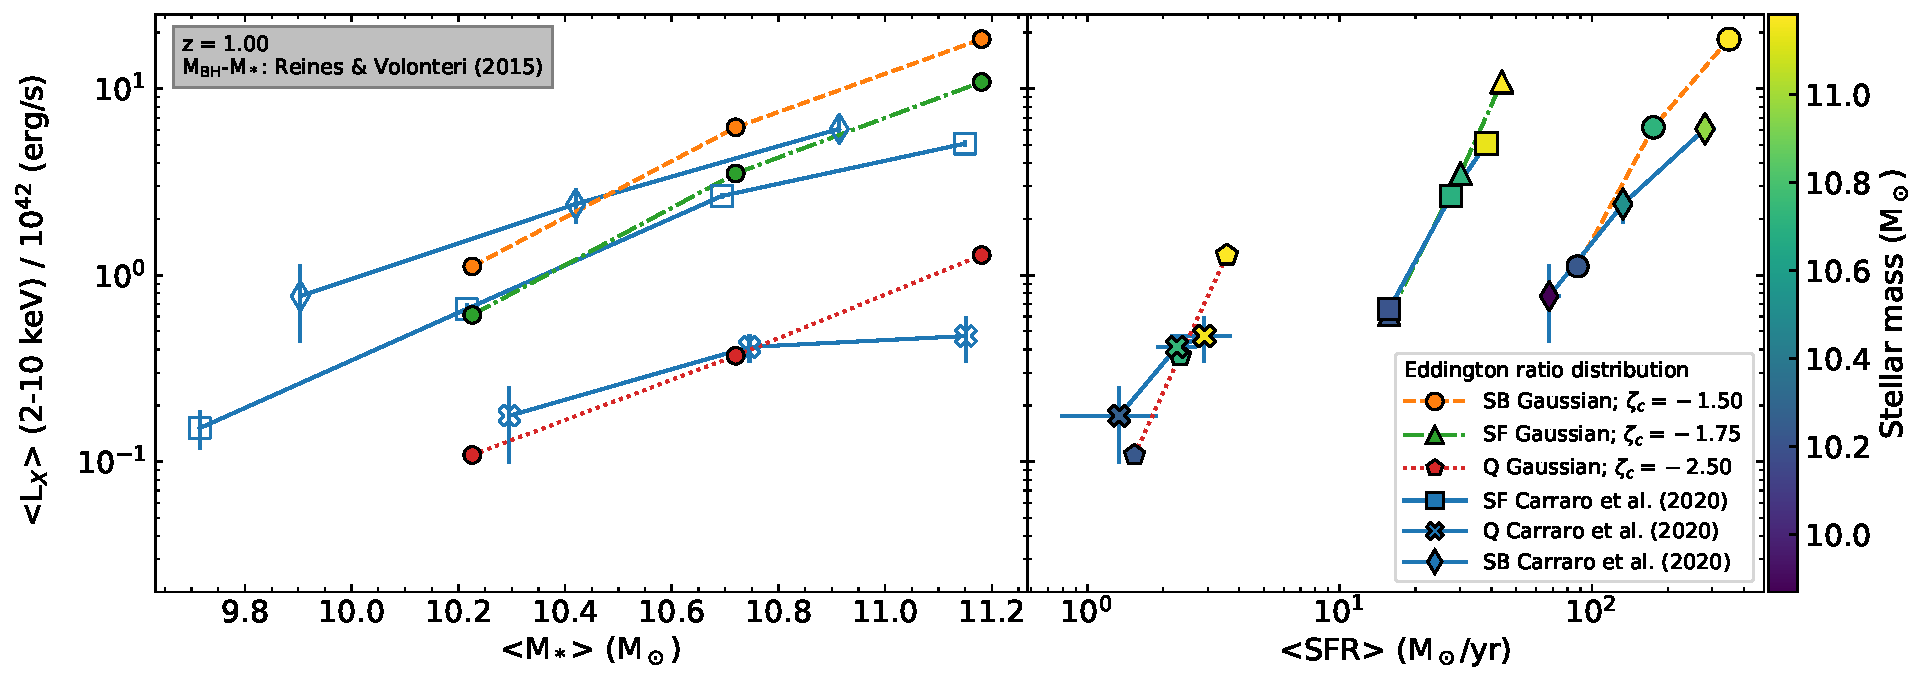
\includegraphics[width=\textwidth]{Figs/Chapter3/fig4.pdf} 
  \caption{L$_{\rm X}$ as a function of ${\rm M}_*$ (left) and SFR (right). L$_{\rm X}$ are obtained at $z=1$ with a \citet{2015ApJ...813...82R} M$_{\rm BH}-{\rm M}_*$ scaling relation and with a Gaussian Eddington ratio distribution as shown in the legend, with a $\sigma=0.3 dex$. In the right panel, SFRs are obtained using the fits from \ref{table:all_fitpar} for starburst (SB) and quiescent (Q) while the fit of Eq.~\ref{eq:SFR} is used for star-forming (SF) galaxies. Data points are color coded according to ${\rm M}_*$. All relations are compared with results from COSMOS data from Chapter~\ref{ch:observations}.}
    \label{fig:SFQSB}
\end{center}
\end{figure*}

\subsection{Reproducing the ${\rm L}_{\rm X}-{\rm M}_*$ relation in starburst, main-sequence and quiescent galaxies} \label{subsec:SFQSB}

In this Section we focus on the dependence of the ${\rm L}_{\rm X}-{\rm M}_*$ relation on galaxy type at fixed redshift, specifically $z=1$.
In Chapter~\ref{ch:observations} we showed in fact that, at least at $z<2.25$, starbursts, star forming and quiescent galaxies are characterized by distinct ${\rm L}_{\rm X}-{\rm M}_*$ relations, which are similar in slope but differ in normalization by a factor of $\sim 10$ when moving from quiescent galaxies, with the lowest average ${\rm L}_{\rm X}$, to the starbursts, with the largest average L$_{\rm X}$ at fixed stellar mass. 

In the left panel of Fig.~\ref{fig:SFQSB} we explore mocks with a constant input ${\rm M}_{\rm BH}-{\rm M}_*$ relation from \citet{2015ApJ...813...82R}, and a varying $\zeta_c$ (circles, triangles, and pentagons) against the different data sets for the three types of galaxies studied in Chapter~\ref{ch:observations} (blue diamonds, squares and crosses for starbursts, star forming, and quiescent galaxies respectively). Reproducing the steep increase in mean ${\rm L}_{\rm X}$ at fixed ${\rm M}_*$ requires, as expected, a proportionally higher value of $\zeta_c$ in star forming and starburst galaxies, assuming the same ${\rm M}_{\rm BH}-{\rm M}_*$ relation.

Interestingly, it is apparent from Fig.~\ref{fig:SFQSB} that the observed ${\rm L}_{\rm X}-{\rm M}_*$ relation is not a simple power law but tends to show a break that becomes more pronounced in more massive quiescent galaxies of mass $\log (M_*/M_{\odot}) \gtrsim 11$. In our modeling this feature could be naturally reproduced with a further decrease in $\zeta_c$ in the most massive and quiescent galaxies in our sample, which would align with the idea of downsizing, supporting the view that more massive galaxies and their central BHs have accreted their mass at a faster pace and are now in their declining phase. We stress that the downsizing in $\zeta_c$ would be even more pronounced if steeper M$_{\rm BH}-{\rm M}_*$ relations were adopted in input. The right panel of Fig.~\ref{fig:SFQSB} shows that our chosen values of $\zeta_c$ that match the ${\rm L}_{\rm X}-{\rm M}_*$ relation for each galaxy type also reproduce, at the same time, their respective ${\rm L}_{\rm X}-{\rm SFR}$ relations, where the SFR is assigned to each galaxy type based on their observed underlying ${\rm M}_*-{\rm SFR}$ relation.

An alternative way to explain the different normalizations of starburst and quiescent galaxies in the ${\rm L}_{\rm X}-{\rm M}_*$ plane would be to adopt the same $\zeta_c$ for all galaxy types and progressively increase the normalization of the M$_{\rm BH}-{\rm M}_*$ scaling relation when moving from quiescent to starburst galaxies.  
However, such a solution would not be favored from an evolutionary point of view as quiescent galaxies should be older galaxies with larger BHs at fixed stellar mass.

All in all, the evolutionary picture that could be extracted from Fig.~\ref{fig:SFQSB} is one in which the central BH and its host galaxy move around a similar M$_{\rm BH}-{\rm M}_*$ scaling relation throughout their lifetime. They could start from a main-sequence or even starburst, gas-rich phase, evolving at an almost constant (specific) SFR, as also proposed by theoretical models \citep[e.g.][]{2014ApJ...782...69L, Aversa15} and direct observations (Chapter~\ref{ch:observations}), and then gradually switch off their accretion and star formation due to internal gas consumption, thus gradually reducing their SFR and accretion onto the central BH (right panel of Fig.~\ref{fig:SFQSB}).  

\section{Discussion and conclusions}\label{sec:disc_concl}
In this Letter we use statistical semi-empirical models to generate accurate mock catalogs of active galaxies, which we analyze in the same manner as in the comparison observational sample from Chapter~\ref{ch:observations}. Our goal is to unveil the input parameters driving the L$_{\rm X}-{\rm M}_*$ relation. We start from a halo mass function at a given redshift, we assign galaxies and BHs to dark matter haloes via the most up-to-date empirical stellar-halo and M$_{\rm BH}-{\rm M}_*$ relations and we assume a SFR depending only on stellar mass and redshift. We explore a range of Eddington ratio distributions, M$_{\rm BH}-{\rm M}_*$ scaling relations and duty cycles.

We show that the L$_{\rm X}$-SFR or L$_{\rm X}-{\rm M}_*$ is largely independent of the AGN duty cycle, but strongly depends on the shape of the M$_{\rm BH}-{\rm M}_*$ scaling relation and on the characteristic Eddington ratio $\zeta_c$, linking the mean L$_{\rm X}$ with the M$_{\rm BH}$. The L$_{\rm X}-{\rm M}_*$ relation can break degeneracies among input duty cycles, Eddington ratio distributions and also BH-galaxy scaling relations, especially when the latter are coupled with AGN clustering measurements \citep{ShankarNat}, thus representing a powerful tool for cosmological models. 
We find that our current data on L$_{\rm X}-{\rm M}_*$ favor, at fixed $\zeta_c$, flatter M$_{\rm BH}-{\rm M}_*$ relations, or M$_*$-dependent $\zeta_c$ for steeper M$_{\rm BH}-{\rm M}_*$ relations. An M$_*$-dependent $\zeta_c$ combined with a steeper M$_{\rm BH}-{\rm M}_*$ relations would indeed be favored by different observational studies \citep[][and Fig.~\ref{fig:comp_models}]{2019ApJ...885L..36D, 2019MNRAS.484.4360A}, continuity equation arguments \citep{Shankar13Acc,Aversa15} and population synthesis models \citep{2018MNRAS.476..436B}. We checked that by fitting the observed L$_{\rm X}-{\rm M}_*$ at $z=1$ with a $P(\log \lambda, z)$ distribution with a characteristic $\zeta_c\simeq-2.15$, is nicely consistent with the mean specific BH accretion rate $\lambda_{sBHAR}$ measured by \citet{2019MNRAS.484.4360A} from large samples of deep X-ray AGN surveys.

In our previous Chapter, see e.g. Fig.~\ref{fig:SF_BH_all}, we showed that main-sequence and quiescent galaxies share similar ratios of BHAR and SFR at all probed cosmic epochs, suggesting that the two processes are linked together throughout different galaxy phases.  
In fact, the mean BHAR/SFR can be written as ${\rm BHAR/SFR} \propto L_{bol}/{\rm SFR} \propto 10^{\zeta_c} {\rm M}_{\rm BH}/(k {\rm M}_*)$, where $k={\rm SFR}/{\rm M}_*$ is the specific SFR. Thus, at fixed ${\rm M}_{\rm BH}/{\rm M}_*$, a similar BHAR/SFR ratio as the one observed in star forming and quiescent galaxies, would be induced by a proportional decline in characteristic Eddington ratio $\zeta_c$ and specific SFR $k$ within a bin of stellar mass. Analogously, the significantly lower BHAR/SFR in starbursts with respect to quiescent/star forming galaxies as measured in Chapter~\ref{ch:observations}, would be naturally interpreted as a proportionally higher specific SFR $k$ %and roughly constant $\zeta_c$ throughout the star formation phase, as predicted by some BH evolution models \citep[e.g.,][]{Aversa15}.
and roughly constant or slightly higher $\zeta_c$ in these young gas rich systems, as predicted by some BH evolution models \citep[e.g.,][]{Aversa15}.